\documentclass{article}
\usepackage{graphicx} % Required for inserting images
\usepackage{amsmath}
\usepackage{amssymb}
\usepackage{enumitem}
\usepackage{placeins}

\title{ECE 760 - Homework 1}
\author{Jed Pulley }
\date{}

\begin{document}

\maketitle

\FloatBarrier
\section*{Problem 1.1}
From \textbf{Topic 2, Definition 2.3} we can see that a subset $U \subseteq \mathbb{R}^D$ is a \textit{subspace} if for every $a, b \in \mathbb{R}$ and every $\textbf{u, v} \in U$, $a\textbf{u} + b\textbf{v} \in U$. Stated another way, a subspace must meet the three requirements below:

\begin{enumerate}
    \item \textbf{Closed under addition:} Let $\mathbf{x} = (x_1, x_2, \dots, x_D)$ and $\mathbf{y} = (y_1, y_2, \dots, y_D)$ be vectors in \(\mathbb{R}^{D}\). 
    Then their sum $\mathbf{x} + \mathbf{y} = (x_1 + y_1, x_2 + y_2, \dots, x_D + y_D)$ is also in \(\mathbb{R}^{D}\). This is because each component of \(\mathbf{x}+\mathbf{y}\) is the sum of two real numbers, which are also real numbers.
    \item \textbf{Closed under scalar multiplication:} Let $\mathbf{x} = (x_1, x_2, \dots, x_D)$ be a vector in \(\mathbb{R}^{D}\) and let \(c\) be a scalar. Then the scalar multiple $c\mathbf{x} = (cx_1, cx_2, \dots, cx_D)$ is also in \(\mathbb{R}^{D}\). This is because each component of \(c\mathbf{x}\) is the product of a real number and a scalar, which is also a real number.
    \item \textbf{Contains the zero vector:} The vector $\mathbf{0} = (0, 0, \dots, 0)$ is in \(\mathbb{R}^{D}\), so \(\mathbb{R}^{D}\) is nonempty. 
\end{enumerate}

\FloatBarrier
\section*{Problem 1.2}
\begin{enumerate}[label=(\alph*)]
    \item To show this, say we have a vector \textbf{x} in $\mathbb{R}^2$
\begin{align}
    \textbf{x} &= \begin{bmatrix}
           1 \\
           -1 \\
         \end{bmatrix}
\end{align}
If we take element-wise square roots of this vector, we get $\sqrt{1}$ equal to 1 and $\sqrt{-1}$ being an imaginary number. Thus, we can show that $\mathbb{R}^D$ is NOT closed under element-wise square roots

    \item An example of a subspace that is closed uner element-wise square roots is $\mathbb{C}^D$
\end{enumerate}

\FloatBarrier
\section*{Problem 1.3}
As stated in Problem 1.1, to show that something is a subspace, we need to satisfy three properties:
\begin{enumerate}
    \item \textbf{Closed under addition:}
    Since our in $\mathbb{R}^D$, then we know that any sort of linear operation will remain in the real number space, thus it's closed under addition
    \item \textbf{Closed under scalar multiplication:}
    The same above applies for scalar multiplication. So long as we scale by a real number, we'll stay in $\mathbb{R}^D$
    \item \textbf{Contains the zero vector:}
    And finally, since our vectors belong to $\mathbb{R}^D$, we know it contains the zero vector. 
\end{enumerate}

Thus we can say that $U = span[\textbf{u}_1, ...,\textbf{u}_R]$ is a subspace

\FloatBarrier
\section*{Problem 1.4}
Let's say that the probability that the genes are inactive is represented as 
\[\mathbb{P}(A|B) = 0.95\]
and that the probability that you have diabetes is represented as 
\[\mathbb{P}(B) = 0.093\]
then using Bayes Rule, we can see that 
\[\mathbb{P}(B|A) = \frac{\mathbb{P}(A|B) \mathbb{P}(B)}{\mathbb{P}(A)}\] 
and filling the known values, we have
\[\mathbb{P}(B|A) = \frac{0.95 * 0.093}{\mathbb{P}(A)}\]

\begin{enumerate}[label=(\alph*)]
  \item An answer cannot be determined given the information.
  \item We would need to know $\mathbb{P}(A)$ which is the percentage of the population has those genes inactive.
  \item Let's just assume that $\mathbb{P}(A) = 0.1$. Meaning that 10\% of the population have those genes inactive, resulting in $\mathbb{P}(B|A) = 0.88$, or, there being an 88\% chance that you have diabetes given you have those genes inactive. Plainly stated, if the inactive genes are exceedingly uncommon among the population without diabetes, I would be very concerned. 88\% is pretty high, I'd be talking to my doctor.
\end{enumerate}

\FloatBarrier
\section*{Problem 1.5}
Considering the observation that larger delays are rarer than shorter ones, the model I chose is the probability density function of the exponential distribution: 

\[t - t_0 \sim \frac{1}{\theta}exp(-\frac{x}{\theta})\] 

Here:
\begin{itemize}
    \item x is our random variable denoting the delay.
    \item $\theta$ is a positive parameter governing the expected delay characteristics, where the larger the value, the longer the delay.
\end{itemize}

The exponential distribution is a suitable model since it is right-skewed. This aligns with the observation that larger delays are rarer than shorter ones.

\FloatBarrier
\section*{Problem 1.6}
\begin{figure}
  \centering
  \begin{minipage}[b]{0.4\textwidth}
    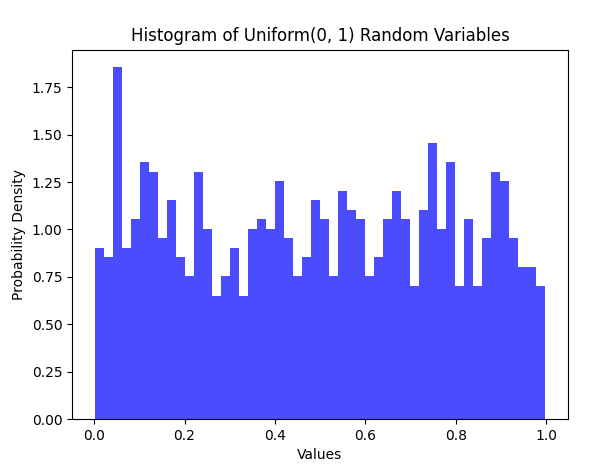
\includegraphics[width=\textwidth]{assets/image.png}
    \caption{Unfirom Distribution}
  \end{minipage}
  \hfill
  \begin{minipage}[b]{0.4\textwidth}
    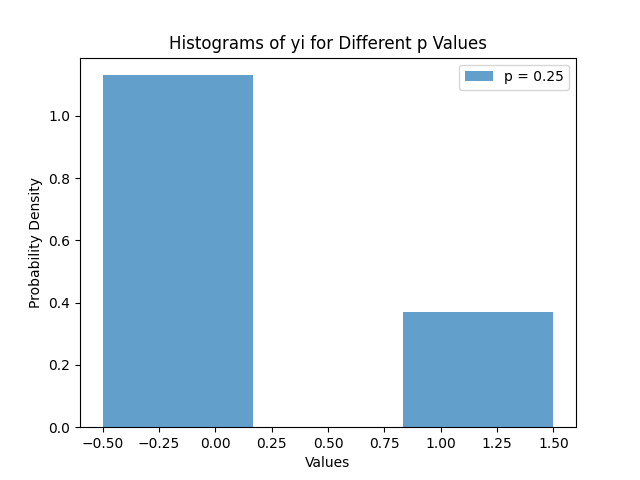
\includegraphics[width=\textwidth]{assets/pvalue1.png}
    \caption{p=0.25}
  \end{minipage}
\end{figure}
\begin{figure}
  \centering
  \begin{minipage}[b]{0.4\textwidth}
    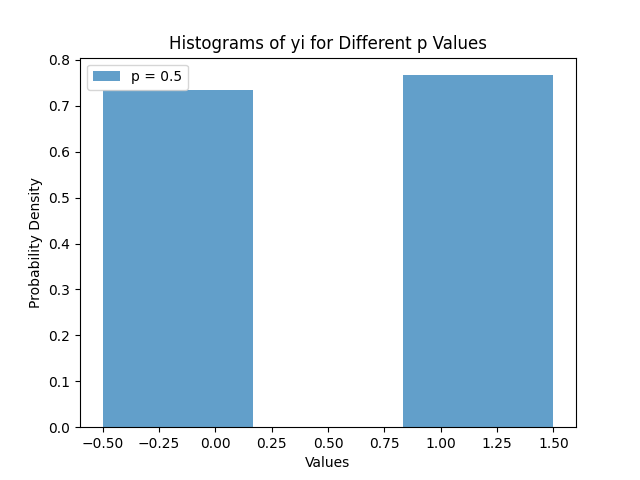
\includegraphics[width=\textwidth]{assets/pvalue2.png}
    \caption{p=0.5}
  \end{minipage}
  \hfill
  \begin{minipage}[b]{0.4\textwidth}
    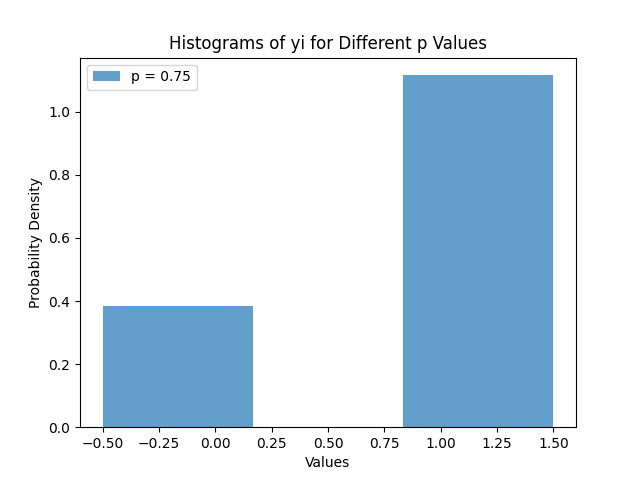
\includegraphics[width=\textwidth]{assets/pvalue3.png}
    \caption{p=0.75}
  \end{minipage}
\end{figure}

\begin{enumerate}[label=(\alph*)]
    \item As shown in in Figure 1 below, I created a small python script using np.random.uniform(0,1,N=1000). Given the randomness, I would say that it is uniform\textbf{-ish}, although it definitely could be better.
    
    \item We can rewrite this as:
    \[\mathbb{P}(y_i = 1) = \mathbb{P}(x_i \le p) = p\]
    \[\mathbb{P}(y_i = 0) = \mathbb{P}(x_i > p) = 1 - p\]
    which shows that $y_i$ is a Bernoulli distribution where p is our threshold, 1 is the probability of success, and 0 is the probability of failure.
    
    \item See figures 2, 3, and above. Yes, they match the expected threshold
    \item If $z_k$ is the sum of a batch of $y_i$'s that are themselves of a Bernoulli distribution, then $z_k$ would follow a Binomial distribution. More formally:
    \[z_k \sim \mathbb{P}(x = \mathrm{x})= 
    \begin{pmatrix} 
      n \\ 
      \mathrm{x} \\ 
    \end{pmatrix}p^\mathrm{x}(1-p)^{n -\mathrm{x}}, \mathrm{x} = 0, \dots, n \]
    \item Using np.random.binomial, it shows that they match (d) fairy closely
\end{enumerate}

\FloatBarrier
\section*{Problem 1.7}
With our regresion model like so:
    \[l(\theta) = \sum_{\mathrm{i} = 1}^{N} [\mathrm{y_i} log(\frac{1}{1+e^{-\theta^T\mathrm{x_i}}}) + (1 - \mathrm{y})log(\frac{1}{1+e^{\theta^T\mathrm{x_i}}})]  \]
\begin{enumerate}[label=(\alph*)]
    \item We can express our gradient like so:
    
    \[\nabla \mathrm{l}(\theta) = \vec{\mathrm{x}}[\sum_{\mathrm{i}=1}{n}(\frac{1-e^{\theta^T\mathrm{x}}}{1+e^{\theta^T\mathrm{x}}}\mathrm{y_i} + \frac{e^{\theta^T\mathrm{x}}}{1+e^{\theta^T\mathrm{x}}})]\]
    
    \item And our Hessian will like so:
    \[ H(l(\theta))= \mathrm{\vec{x}\vec{x}^T}\sum_{k=1}^{n}\frac{(1-2\mathrm{y_k})e^{\theta^T\mathrm{x}}}{(1+e^{\theta^T\mathrm{x}})^2} \]
    \item As such, $l(\theta)$ is a scalar, $\nabla \mathrm{l}(\theta)$ is a vector, and $H(\mathrm{l}(\theta))$ is a matrix
\end{enumerate}

\end{document}